\documentclass{standalone}
\usepackage{tikz}
\usepackage{forest}
\usepackage{xcolor}
\def\es{edge from parent[solid]}
\def\ed{edge from parent[dashed]}
%\definecolor{fpgreen}{HTML}{A6D609}
\definecolor{fpgray}{HTML}{7B7B7C}
\def\edm{edge from parent[dashed] [fpgray] node[auto=left] {\scriptsize ?} }
\begin{document}	
\centering
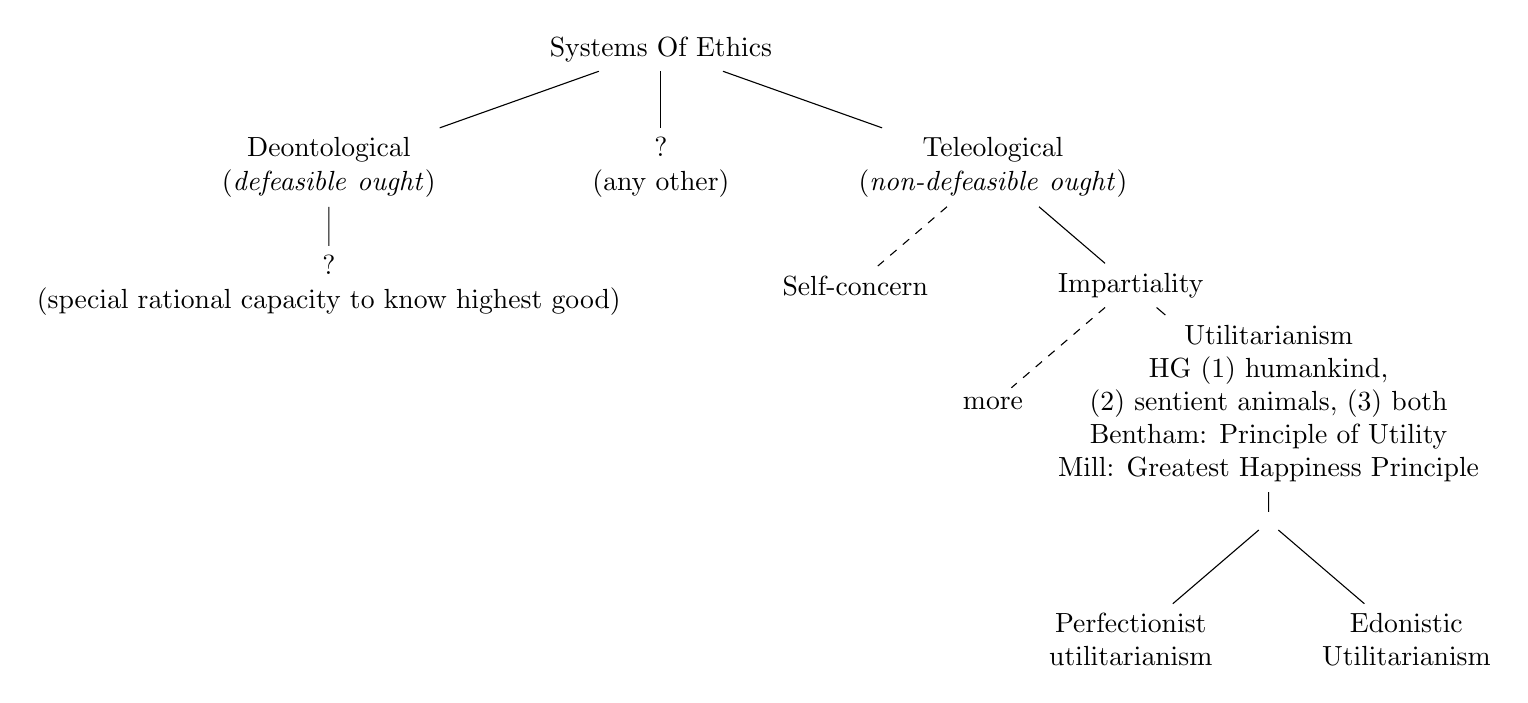
\begin{tikzpicture}[every node/.style={align=center},level 1/.style={sibling distance=12em},level 2/.style={sibling distance=35mm}, level 3/.style={sibling distance=30mm} level 4/.style={sibling distance=30mm}
]
\node {Systems Of Ethics}
    [sibling distance=6cm]
child { node {Deontological \\ (\textit{defeasible} \textit{ought})} 
child { node {? \\ (special rational capacity to know highest good)}}} % <- End Deontological
child { node {? \\ (any other)} }
child { node {Teleological \\ (\textit{non-defeasible} \textit{ought})} child {node {Self-concern} \ed} child {node {Impartiality} child {node {more} \ed} 
child {node {Utilitarianism \\ HG (1) humankind, \\ (2) sentient animals, (3) both \\ Bentham: Principle of Utility \\ Mill: Greatest Happiness Principle}
child {node [] {} 
child {node {Perfectionist \\ utilitarianism} }
child {node {Edonistic \\ Utilitarianism}}}} }}
;
\end{tikzpicture}
\end{document}